In this chapter, we will discuss the performance of our approach towards neural networks.
We will explore various options available through our approach to elicit optimal results.
To achieve this, the evaluation will be based on the following research questions:
\begin{enumerate}
    \item[]\textbf{RQ1: Impact of Training on Mutated Models} How does training a mutated pre-trained model impact its performance metrics?
    \item[]\textbf{RQ2: Effects of Mutation Without Training} What is the effect on performance metrics when a pre-trained model is mutated without further training?
    \item[]\textbf{RQ3: Training Dataset Size and Approach Performance} What is the impact of the size of the training dataset on the approach's effectiveness?
    \item[]\textbf{RQ4: Influence of Suspiciousness Measures} How do different suspiciousness measures influence the outcomes of the experiments?
    \item[]\textbf{RQ5: CNN vs. DNN Architectural Efficiency} Which architecture yields better results for our approach: CNN or DNN?
    \item[]\textbf{RQ6: Offset Variations in Loss and Accuracy} How do variations in offset for loss and accuracy affect the approach's performance?
    \item[]\textbf{RQ7: Break Conditions and Algorithm Performance} What is the effect of different break conditions on the efficiency and effectiveness of the algorithm?
    \item[]\textbf{RQ8: Contributions of Different Mutation Functions} How do different mutation functions contribute to the model's performance with our Algorithm?
\end{enumerate}
\section{Setup}\label{sec:setup}

We evaluated our approach on a Workstation consisting of an AMD Ryzen 9 3900X 12-Core Processor 4,6 GHz, with 32 GB of RAM and an NVIDIA GeForce RTX 4070Ti GPU with 12 GB of VRAM and 7680 CUDA Cores.
The setup is running Ubuntu release 22.04, running with Windows Subsystem for Linux, on Microsoft Windows 11 Pro, we use it because since version 2.11\cite{noauthor_build_2023} TensorFlow doesn't support GPU acceleration natively any more.
Regarding the Software, we are using Python version 3.10.12 and using TensorFlow version 2.14.1, with CUDA version 12.3.

\subsection*{Architecture}
We are using the Fashion-MNIST dataset\cite{xiao_fashion-mnist_2017} for our experiments, which consists of 60,000 training images and 10,000 test images, each of size 28×28 pixels, with 10 classes.
For the evaluation we haven't used not only the whole, but also a half and a quarter of the training data, which are derived from the original training data, by using Scikit-learn's\cite{pedregosa_scikit-learn_2011} \texttt{train\_test\_split} function, with a test size of 0.5 and 0.75 respectively.

We used 2 DNNs and 2 CNNs, in the following table \ref{tab:architecture} a plain number describes the number of neurons in a dense layer. $CL$ describes a combination of a convolutional layer with a stride of $(1,1)$ and a kernel size of $(3,3)$ and a pooling layer with a pool size of $(2,2)$. We used.
Adam as our optimizer with a learning rate of 0.001.
% Please add the following required packages to your document preamble:
% \usepackage{multirow}
% \usepackage{lscape}
% Please add the following required packages to your document preamble:
% \usepackage{multirow}
\begin{table}[htbp]
    \centering
    \caption{Overview of Neural Network Architectures used for evaluation}
    \begin{tabular}{|c|c|c|}
        \hline
        Model Name            & Mod. Param.         & Architecture                 \\ \hline
        \multirow{2}{*}{DNN1} & \multirow{2}{*}{16} & \multirow{2}{*}{$<16>$}      \\
        &                     &                              \\ \hline
        \multirow{2}{*}{DNN2} & \multirow{2}{*}{64} & \multirow{2}{*}{$<4x16>$}    \\
        &                     &                              \\ \hline
        \multirow{2}{*}{CNN1} & \multirow{2}{*}{12} & \multirow{2}{*}{$<CL,4>$}    \\
        &                     &                              \\ \hline
        \multirow{2}{*}{CNN2} & \multirow{2}{*}{20} & \multirow{2}{*}{$<CL,CL,4>$} \\
        &                     &                              \\ \hline
    \end{tabular}
    \label{tab:archi}
\end{table}
\begin{table}[htbp]
    \centering
    \caption{Results of the initial Training of the different models}
    \begin{tabular}{|cc|ccc|ccc|}
        \hline
        \multicolumn{2}{|c|}{Model} & \multicolumn{3}{c|}{Accuracy} & \multicolumn{3}{c|}{Loss} \\ \hline
        \multicolumn{1}{|c|}{Name}                  & Init. Epochs & \multicolumn{1}{c|}{Full}    & \multicolumn{1}{c|}{Half}    & Quarter & \multicolumn{1}{c|}{Full}    & \multicolumn{1}{c|}{Half}     & Quarter  \\ \hline
        \multicolumn{1}{|c|}{\multirow{2}{*}{DNN1}} & 1              & \multicolumn{1}{c|}{82.84\%} & \multicolumn{1}{c|}{81.49\%} & 78.65\% & \multicolumn{1}{c|}{49.11\%} & \multicolumn{1}{c|}{53.46\%}  & 62.00\%  \\ \cline{2-8}
        \multicolumn{1}{|c|}{}                      & 6              & \multicolumn{1}{c|}{84.23\%} & \multicolumn{1}{c|}{83.76\%} & 83.57\% & \multicolumn{1}{c|}{44.42\%} & \multicolumn{1}{c|}{44.48\%}  & 46.94\%  \\ \hline
        \multicolumn{1}{|c|}{\multirow{2}{*}{DNN2}} & 1              & \multicolumn{1}{c|}{80.46\%} & \multicolumn{1}{c|}{79.20\%} & 75.97\% & \multicolumn{1}{c|}{54.05\%} & \multicolumn{1}{c|}{57.90\%}  & 66.21\%  \\ \cline{2-8}
        \multicolumn{1}{|c|}{}                      & 6              & \multicolumn{1}{c|}{83.52\%} & \multicolumn{1}{c|}{83.04\%} & 82.74\% & \multicolumn{1}{c|}{44.23\%} & \multicolumn{1}{c|}{46.79\%}  & 48.88\%  \\ \hline
        \multicolumn{1}{|c|}{\multirow{2}{*}{CNN1}} & 1              & \multicolumn{1}{c|}{74.34\%} & \multicolumn{1}{c|}{77.31\%} & 42.62\% & \multicolumn{1}{c|}{72.88\%} & \multicolumn{1}{c|}{66.83\%}  & 147.63\% \\ \cline{2-8}
        \multicolumn{1}{|c|}{}                      & 6              & \multicolumn{1}{c|}{83.69\%} & \multicolumn{1}{c|}{82.14\%} & 61.06\% & \multicolumn{1}{c|}{48.44\%} & \multicolumn{1}{c|}{47.35\%}  & 95.61\%  \\ \hline
        \multicolumn{1}{|c|}{\multirow{2}{*}{CNN2}} & 1              & \multicolumn{1}{c|}{70.49\%} & \multicolumn{1}{c|}{54.52\%} & 63.20\% & \multicolumn{1}{c|}{80.13\%} & \multicolumn{1}{c|}{111.68\%} & 100.31\% \\ \cline{2-8}
        \multicolumn{1}{|c|}{}                      & 6              & \multicolumn{1}{c|}{78.43\%} & \multicolumn{1}{c|}{77.37\%} & 74.56\% & \multicolumn{1}{c|}{60.28\%} & \multicolumn{1}{c|}{59.29\%}  & 65.74\%  \\ \hline
    \end{tabular}
    \label{tab:results}
\end{table}
\subsection*{Parameters}
Fo our evaluation we used the following parameters:
\begin{enumerate}
    \item[]\textbf{Similarity coefficient:} tarantula, dstar with value 3, ochiai and random
    \item[]\textbf{Mutation functions:} \texttt{modify\_weight\_one\_random\_gauss,\\ modify\_weight\_all\_random\_gauss, modify\_bias, modify\_bias\_random\_gauss, modify\_all\_weights, modify\_all\_weights\_by\_scalar,\\modify\_all\_weights\_by\_scalar\_random\_gauss,\\modify\_weight\_all\_random\_by\_scalar\_gauss}
    \item[]\textbf{Break conditions:} loss, accuracy, loss and accuracy, loss or accuracy
    \item[]\textbf{Loss offset:} 0.005, 0
    \item[]\textbf{Accuracy offset:} 0.01, 0
    \item[]\textbf{Loss and accuracy regression:} True for all runs
    \item[]\textbf{Values:} -1, -0.5, 0, 0.5, 1 \textit{0 just for value assignment, basically a deletation of a neuron}
    \item[]\textbf{Sigma for random:} 0.5, 1
\end{enumerate}
\section{Impact of Training on Mutated Models}\label{sec:impact-of-training-on-mutated-models}
\begin{figure}
    \centering
    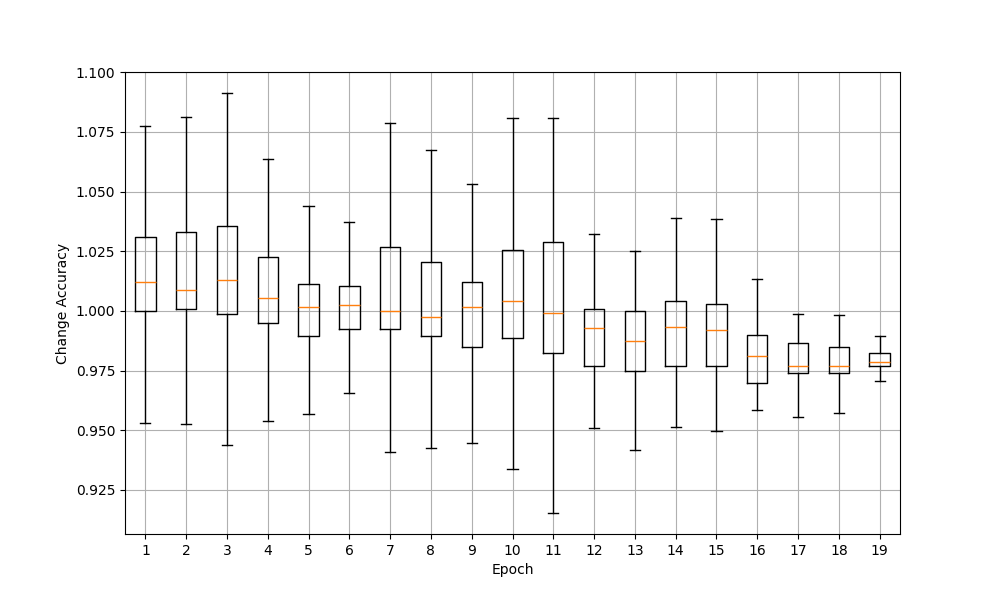
\includegraphics[width=\textwidth]{plots/Trained_Change_Acc.png}
    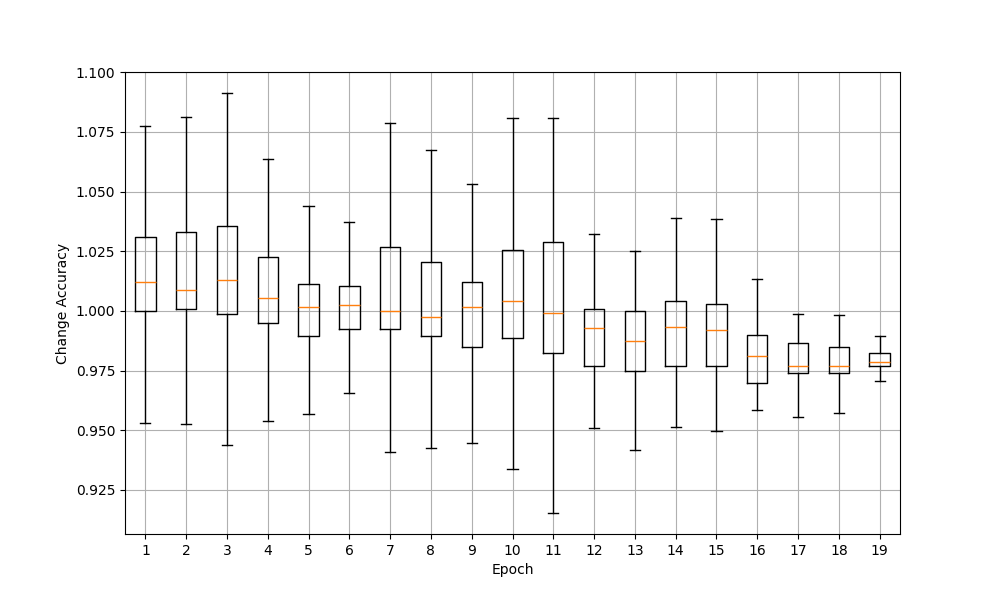
\includegraphics[width=\textwidth]{plots/Trained_Change_Loss.png}
    \caption{Loss and accuracy of the models, with training}
    \label{fig:loss-accuracy-training}
\end{figure}
\begin{figure}
    \centering
    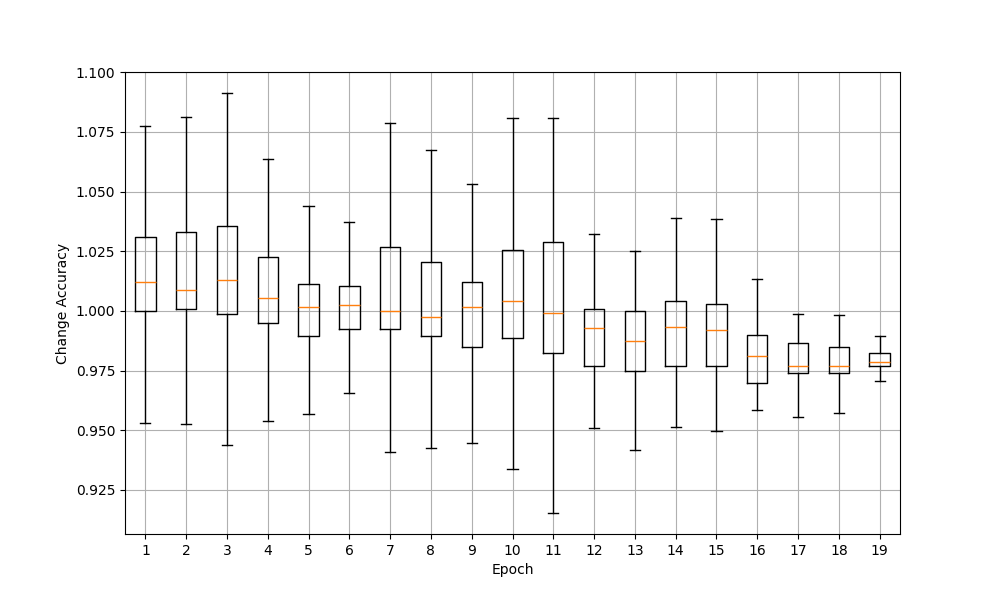
\includegraphics[width=\textwidth]{plots/Trained_Points_perEpoch.png}
    \caption{Decay of data points, per epoch, with training}
    \label{fig:decay_training}
\end{figure}
\section{Effects of Mutation Without Training}\label{sec:effects-of-mutation-without-training}
\begin{figure}
    \centering
    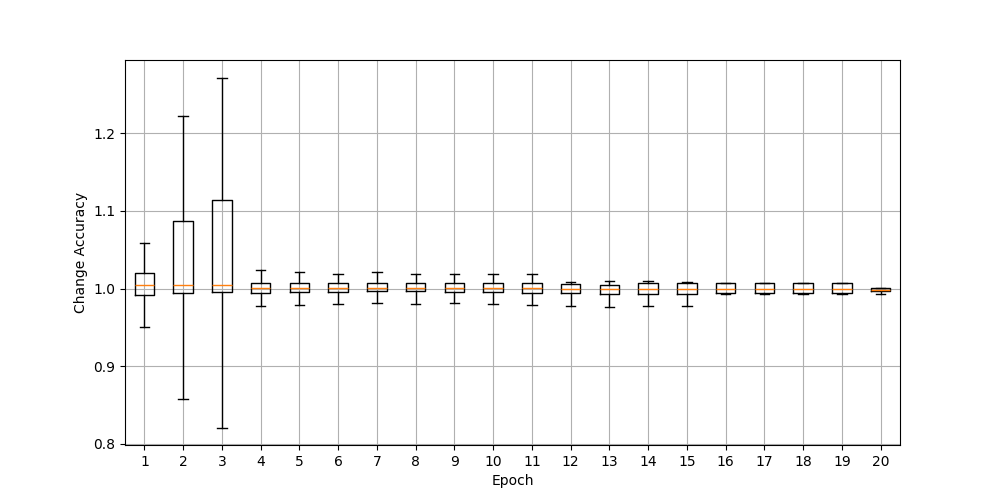
\includegraphics[width=\textwidth]{plots/NotTrained_Change_Acc.png}
    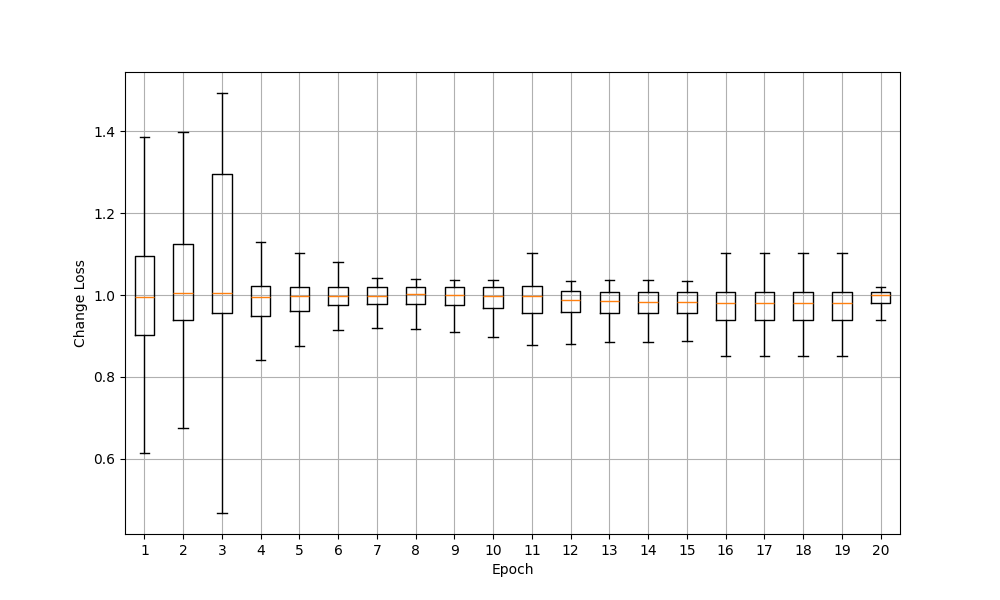
\includegraphics[width=\textwidth]{plots/NotTrained_Change_Loss.png}
    \caption{Loss and accuracy of the models, without training}
    \label{fig:loss-accuracy-Notraining}
\end{figure}
\begin{figure}
    \centering
    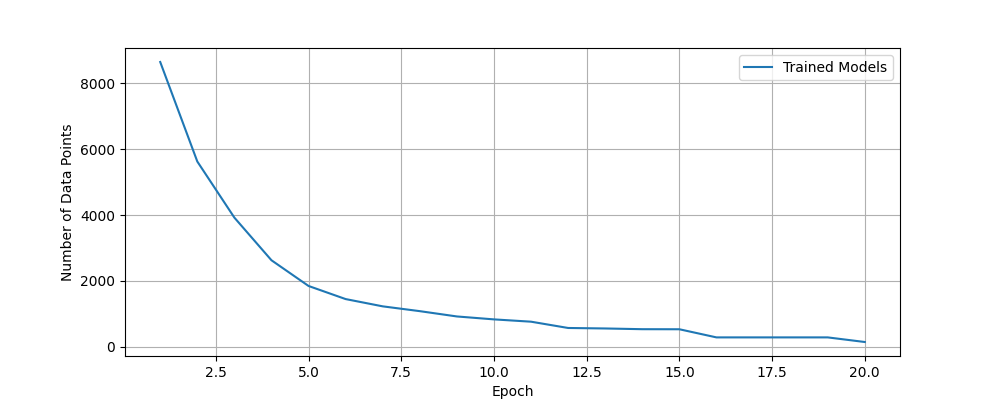
\includegraphics[width=\textwidth]{plots/NotTrained_Points_perEpoch.png}
    \caption{Decay of data points, per epoch, without training}
    \label{fig:decay_Notraining}
\end{figure}
\section{Training Dataset Size and Model Performance}\label{sec:training-dataset-size-and-model-performance}
\begin{figure}
    \begin{subfigure}{0.5\textwidth}
        \centering
        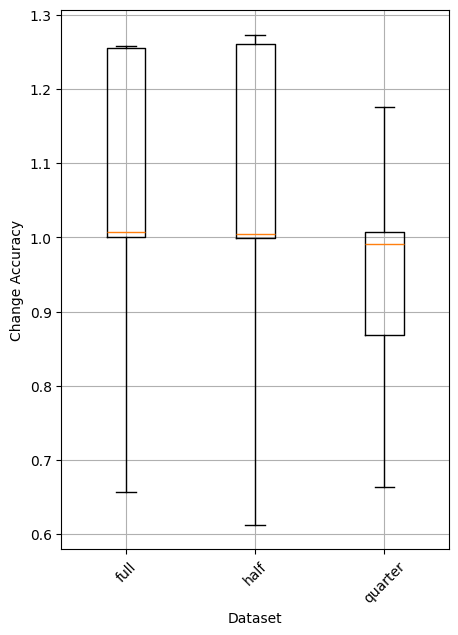
\includegraphics[width=0.95\textwidth]{plots/Dataset_NotTrained_accuracy.png}
    \end{subfigure}
    \begin{subfigure}{0.5\textwidth}
        \centering
        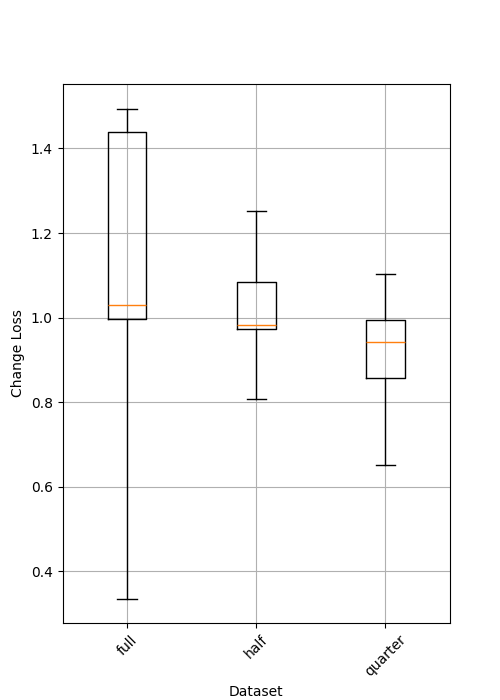
\includegraphics[width=0.95\textwidth]{plots/Dataset_NotTrained_loss.png}
    \end{subfigure}
    \caption{Loss and accuracy, without training, with different dataset sizes}
    \label{fig:dataset-size-notraining}
\end{figure}
\begin{figure}
    \begin{subfigure}{0.5\textwidth}
        \centering
        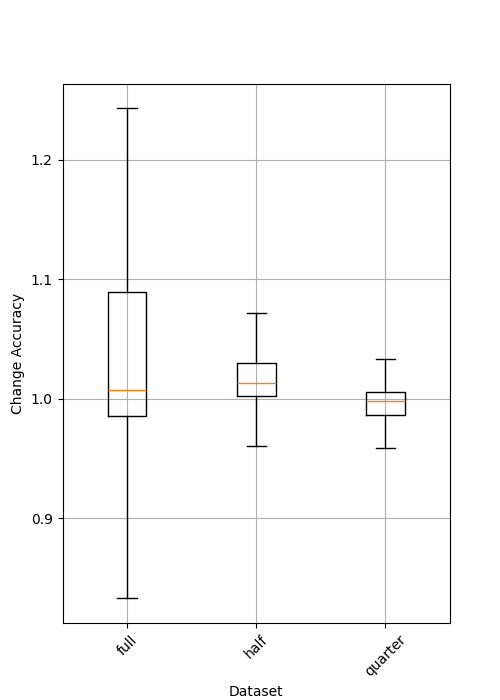
\includegraphics[width=0.95\textwidth]{plots/Dataset_Trained_accuracy.png}
    \end{subfigure}
    \begin{subfigure}{0.5\textwidth}
        \centering
        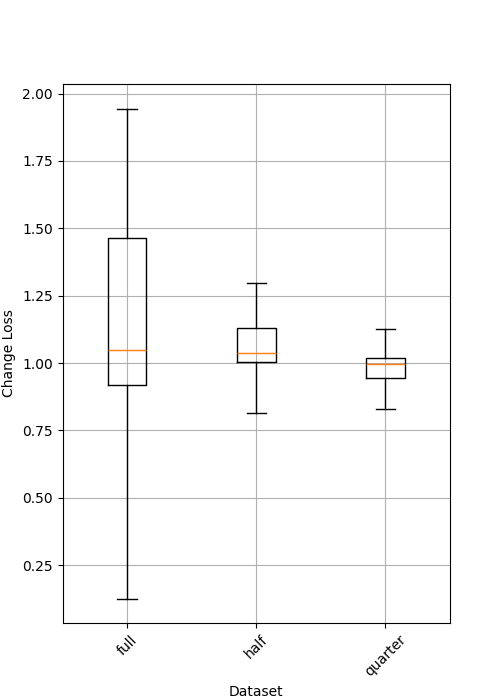
\includegraphics[width=0.95\textwidth]{plots/Dataset_Trained_loss.png}
    \end{subfigure}
    \caption{Loss and accuracy, with training, with different dataset sizes}
    \label{fig:dataset-size-training}
\end{figure}
\section{Influence of Suspiciousness Measures}\label{sec:influence-of-suspiciousness-measures}


\section{CNN vs. DNN Architectural Efficiency}\label{sec:cnn-vs.-dnn-architectural-efficiency}


\section{Offset Variations in Loss and Accuracy}\label{sec:offset-variations-in-loss-and-accuracy}


\section{Break Conditions and Algorithm Performance}\label{sec:break-conditions-and-algorithm-performance}


\section{Contributions of Different Mutation Functions}\label{sec:contributions-of-different-mutation-functions}